%% ============================================================
%% LegalShadow — ICI2ST 2026 · MDPI Engineering Proceedings template
%% Compile: pdflatex paper && bibtex paper && pdflatex paper && pdflatex paper
%% ============================================================
\documentclass[engproc,article,submit,moreauthors]{Definitions/mdpi}

\usepackage{tikz}
\usetikzlibrary{arrows.meta,positioning,shapes.geometric,fit,backgrounds,calc}
\usepackage{pgfplots}
\pgfplotsset{compat=1.17}
\usepgfplotslibrary{polar}
\usepackage{xcolor}

%% ── Colour palette ─────────────────────────────────────────
\definecolor{lsBlue}{HTML}{2563EB}   % acquisition / observed
\definecolor{lsCyan}{HTML}{0891B2}   % semantic
\definecolor{lsViolet}{HTML}{7C3AED} % validation
\definecolor{lsAmber}{HTML}{D97706}  % presentation
\definecolor{lsGreen}{HTML}{059669}  % covered / evidence present
\definecolor{lsRed}{HTML}{DC2626}    % gap / missing
\definecolor{lsSlate}{HTML}{475569}  % neutral

%% MDPI internal commands - do not modify
\firstpage{1}
\makeatletter
\setcounter{page}{\@firstpage}
\makeatother
\pubvolume{1}
\issuenum{1}
\articlenumber{0}
\pubyear{2026}
\copyrightyear{2026}
\datereceived{ }
\daterevised{ }
\dateaccepted{ }
\datepublished{ }

%% ── Title ──────────────────────────────────────────────────
\Title{LegalShadow: An Ontology-Guided Digital Shadow Architecture via JSON-LD for Automated Semantic Validation of LegalTech Ecosystems}

\newcommand{\orcidauthorA}{0000-0001-6285-7390} % P.M. Paccha-Angamarca
\newcommand{\orcidauthorB}{0000-0003-2916-0369} % E.J. Sacoto-Cabrera
\newcommand{\orcidauthorC}{0000-0002-7335-2571} % V.V. Velepucha-Bonett

\Author{
    Patricio M. Paccha-Angamarca $^{1,2,}$*\orcidA{},
    Erwin J. Sacoto-Cabrera $^{2}$\orcidB{} and
    V\'ictor V. Velepucha-Bonett $^{1}$\orcidC{}
}
\AuthorNames{
    Patricio M. Paccha-Angamarca,
    Erwin J. Sacoto-Cabrera and
    V\'ictor V. Velepucha-Bonett
}
\address{
    $^{1}$ \quad Software Engineering Creation, Application and Management Group (GI-CreAGSoft),
    National Polytechnic School, Ladr\'on de Guevara E11-253, Quito 170525, Ecuador;
    victor.velepucha@epn.edu.ec\\
    $^{2}$ \quad Cloud Computing, Smart Cities \& High-Performance Computing Group (GIHP4C),
    Salesian Polytechnic University, Calle Vieja 12-30, Cuenca 010105, Ecuador;
    esacoto@ups.edu.ec
}
\corres{Correspondence: patricio.paccha@epn.edu.ec}


%% ── Abstract ───────────────────────────────────────────────
\abstract{The digital transformation of judiciaries produces heterogeneous technological ecosystems whose governance maturity is rarely auditable in an automated, reproducible and semantically grounded way. This paper presents \emph{LegalShadow}, an ontology-guided digital shadow architecture that automatically builds a JSON-LD structural representation of a judicial institution's public digital ecosystem and validates it against a multi-standard governance ontology (TOGAF, COBIT, ITIL, NIST CSF, AI, DLT, open data, security, interoperability and a LegalTech domain). The approach is formalised as the quintuple $\mathcal{M}=\langle \Omega, \Delta, \Gamma, \Psi, \delta \rangle$, where the hierarchical coverage function $\Psi$ quantifies the degree to which the shadow materialises each ontological dimension and the gap function $\delta$ prioritises remediation; boundedness, monotonicity and saturation are established. A containerised implementation was exercised on the Ecuadorian Judiciary Council over 17 dated acquisition runs (2 July--4 August 2026, 187 read-only requests, 170 cryptographically verified snapshots, 0 hash mismatches). The generated shadow (34 components, 32 flows, 7 layers) yields an institutional maturity index of 46/100 (Level 3, ``Defined''), while the ten-dimension semantic validation exposes a global coverage of only $\Psi_{\mathrm{global}}=34.9\%$ (25.8 of 73.9 ontological points), against $90.5\%$ for a synthetic control shadow that saturates the engine. Sensitivity analysis over the weight $w_r \in [0.10, 0.90]$ leaves the remediation agenda stable. The contrast between the optimistic self-reported maturity index and the low semantic coverage is the paper's central empirical finding: declarative digitalisation does not entail machine-actionable governance.}

\keyword{digital shadow; digital twin; ontology; JSON-LD; LegalTech; e-government; open judicial data; semantic web; digital maturity; software architecture}

\begin{document}

%% ============================================================
\section{Introduction}
\label{sec:intro}

Judicial systems worldwide, and in Latin America in particular, are undergoing accelerated digitalisation that combines institutional portals, case management systems, citizen consultation services and statistical repositories. The result is a heterogeneous technological ecosystem in which modern single-page applications (SPA), generic content management systems and legacy applications coexist, with uneven interoperability and scarce exposure of structured data. The e-justice literature has documented that such projects exhibit specific risk factors---organisational complexity, vendor dependence and system fragmentation---that hinder their evaluation and governance \cite{Rosa2013}. In parallel, open government data research consistently reports a gap between the nominal publication of information and its effective reuse through machine-readable formats \cite{Janssen2012,Attard2015}.

Cyber-physical systems engineering has meanwhile consolidated the digital twin paradigm and its variants. The taxonomy of Kritzinger et al. distinguishes digital model, digital shadow and digital twin according to the degree of automation of the information flow between the physical object and its virtual counterpart \cite{Kritzinger2018}: in the \emph{digital shadow} the real-to-virtual flow is automatic, whereas feedback towards the object remains under human control. This configuration is precisely the appropriate one for the judicial domain, where acting upon the ``object'' (public institutional infrastructure) is an exclusive competence of the state and any automatic intervention would be improper; the value of the artefact lies in observation, diagnosis and recommendation. Although the paradigm originated in manufacturing \cite{Tao2019,Jones2020,Fuller2020,Semeraro2021}, its extension to organisations, cities and public services is an active research area \cite{Shahat2021,BotinSanabria2022,Brauner2022}. However, the systematic review by Karabulut et al. on ontologies in digital twins finds that semantic integration remains the weak link: most twins lack a formal conceptual model that endows their data with shared meaning, and---critically for this work---there is no established method to \emph{verify} that a twin actually materialises its semantic model \cite{Karabulut2024}.

The legal domain has a solid tradition in knowledge representation---legal ontologies, normative markup standards and automated legal reasoning \cite{BenchCapon2012,Casanovas2016}---as well as machine learning applied to judicial decision prediction \cite{Katz2017,Medvedeva2020}. Nevertheless, to the best of our knowledge no published architecture (i) automatically builds a structural digital shadow of a judicial institution's technological ecosystem from public web evidence, (ii) serialises it as a knowledge graph in JSON-LD anchored to a governance ontology, and (iii) validates it quantitatively through a hierarchical coverage metric with maturity interpretation. This is the gap addressed here.

The contributions of this paper are four:

\begin{enumerate}
\item \textbf{Formal model.} The quintuple $\mathcal{M}=\langle \Omega, \Delta, \Gamma, \Psi, \delta \rangle$ (Section~\ref{sec:formal}) integrating a reference ontology, an architectural graph, a semantic anchoring function, a hierarchical coverage function and a gap function, with established boundedness, monotonicity and saturation properties.
\item \textbf{Reference architecture.} \emph{LegalShadow}, a containerised four-layer architecture whose acquisition module turns public web signals into a JSON-LD digital shadow conformant to standard vocabularies (Section~\ref{sec:arch}).
\item \textbf{Auditable acquisition protocol.} A non-invasive, read-only, identified evidence collection procedure with per-snapshot SHA-256 manifests and a hash-chained append-only ledger, aligned with the legal and ethical recommendations on web scraping \cite{Krotov2020} and with FAIR data stewardship \cite{Wilkinson2016}.
\item \textbf{Empirical validation.} Application to the Ecuadorian Judiciary Council across 17 dated runs, with a quantified contrast between declarative maturity and machine-actionable semantic coverage, plus sensitivity analysis and a cross-institutional portability probe (Section~\ref{sec:results}).
\end{enumerate}

%% ============================================================
\section{Related Work}
\label{sec:related}

\subsection{Models, Shadows and Twins}
The conceptual distinction between digital model, digital shadow and digital twin proposed by Kritzinger et al. \cite{Kritzinger2018} has become the dominant classification criterion (Figure~\ref{fig:dmdsdt}). Jones et al. identify the twinning process, fidelity and synchronisation rate as defining parameters \cite{Jones2020}; Tao et al. document the industrial state of the art \cite{Tao2019}; and Fuller et al. and Semeraro et al. systematise enabling technologies and open challenges \cite{Fuller2020,Semeraro2021}. Sepasgozar argues that terminological confusion between twin and shadow delays adoption and calls for delimiting both artefacts \cite{Sepasgozar2021}, while the Internet of Production cluster develops the digital shadow as a ``purpose-driven data view''---task-specific data aggregates contextualised by domain models \cite{Brauner2022}. Outside manufacturing, reviews of urban twins \cite{Shahat2021} and general applications \cite{BotinSanabria2022} confirm the expansion of the paradigm into the public sector, yet without instantiations in the judicial domain.

\subsection{Ontologies and Semantics in Digital Twins}
Ontological engineering provides the conceptual apparatus for endowing twins with shared semantics: from the classical definition of an ontology as an explicit specification of a conceptualisation \cite{Gruber1993}, through construction and evaluation methodologies \cite{Uschold1996,Guarino2002}, to contemporary knowledge graphs \cite{Hogan2021}. Karabulut et al. review the use of ontologies in digital twins and conclude that formal validation of the correspondence between the semantic model and the represented system is an open problem \cite{Karabulut2024}; the $\Psi$ function proposed here responds directly to that gap. Regarding serialisation, linked data principles \cite{Bizer2009}, the evolution of the semantic web field \cite{Hitzler2021} and the Schema.org experience with structured data embedded in the web \cite{Guha2016} support the choice of JSON-LD as the interchange format: idiomatic JSON for developers and, simultaneously, RDF for reasoners.

\subsection{Legal Semantic Web and Open Judicial Data}
The AI and Law community has produced core legal ontologies, normative identification standards and legal knowledge management architectures \cite{BenchCapon2012,Casanovas2016}. Machine learning over judicial corpora has demonstrated predictive capability in supreme and international courts \cite{Katz2017,Medvedeva2020}, but presupposes accessible and structured data. Open government research shows that adoption barriers---non-processable formats, absence of APIs, poor metadata---limit the public value of portals \cite{Janssen2012,Attard2015}, and e-justice information systems add their own organisational risks \cite{Rosa2013}. Web extraction is, in practice, the only available mechanism to observe these ecosystems externally, which demands explicit legal and ethical protocols \cite{Krotov2020} and data management objectives aligned with FAIR principles \cite{Wilkinson2016}. Table~\ref{tab:related} positions the contribution against the closest lines of work.

\begin{table}[H]
\small
\caption{Comparison with adjacent research lines. DS: digital shadow; KG: knowledge graph.\label{tab:related}}
\begin{tabularx}{\textwidth}{lCCCC}
\toprule
\textbf{Approach} & \textbf{Judicial domain} & \textbf{Governance ontology} & \textbf{Auto-generated DS} & \textbf{Coverage metric}\\
\midrule
Manufacturing twins \cite{Tao2019,Jones2020} & No & Partial & No & No\\
Urban twins \cite{Shahat2021,BotinSanabria2022} & No & Partial & Partial & No\\
IoP digital shadows \cite{Brauner2022} & No & Yes & Partial & No\\
Ontologies in DT \cite{Karabulut2024} & No & Yes & No & Open problem\\
Legal semantic web \cite{Casanovas2016} & Yes & Partial & No & No\\
\textbf{LegalShadow (this work)} & \textbf{Yes} & \textbf{Yes} & \textbf{Yes} & \textbf{Yes ($\Psi$, $\delta$)}\\
\bottomrule
\end{tabularx}
\end{table}

\begin{figure}[H]
\centering
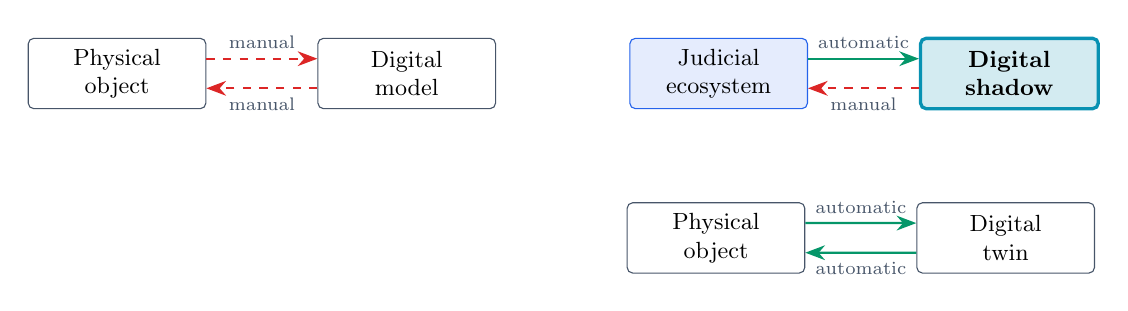
\begin{tikzpicture}[scale=0.94, transform shape,
  obj/.style={draw=lsSlate, rounded corners=2pt, minimum width=2.4cm, minimum height=0.95cm, align=center, font=\small},
  auto/.style={-{Stealth[length=2.5mm]}, thick, lsGreen},
  man/.style={-{Stealth[length=2.5mm]}, thick, dashed, lsRed},
  lab/.style={font=\scriptsize, midway, text=lsSlate}]
\node[obj] (p1) {Physical\\object};
\node[obj, right=1.5cm of p1] (v1) {Digital\\model};
\draw[man] ([yshift=2mm]p1.east) -- node[lab, above]{manual} ([yshift=2mm]v1.west);
\draw[man] ([yshift=-2mm]v1.west) -- node[lab, below]{manual} ([yshift=-2mm]p1.east);
\node[obj, right=1.8cm of v1, fill=lsBlue!12, draw=lsBlue] (p2) {Judicial\\ecosystem};
\node[obj, right=1.5cm of p2, fill=lsCyan!18, draw=lsCyan, very thick] (v2) {\textbf{Digital}\\\textbf{shadow}};
\draw[auto] ([yshift=2mm]p2.east) -- node[lab, above]{automatic} ([yshift=2mm]v2.west);
\draw[man] ([yshift=-2mm]v2.west) -- node[lab, below]{manual} ([yshift=-2mm]p2.east);
\node[obj, below=1.25cm of $(p2.south)!0.5!(v2.south)$, xshift=-2.0cm] (p3) {Physical\\object};
\node[obj, right=1.5cm of p3] (v3) {Digital\\twin};
\draw[auto] ([yshift=2mm]p3.east) -- node[lab, above]{automatic} ([yshift=2mm]v3.west);
\draw[auto] ([yshift=-2mm]v3.west) -- node[lab, below]{automatic} ([yshift=-2mm]p3.east);
\end{tikzpicture}
\caption{Classification of virtual counterparts by information flow (adapted from \cite{Kritzinger2018}). In the judicial domain automatic feedback onto institutional infrastructure is improper, so the digital shadow (shaded) is the correct configuration.\label{fig:dmdsdt}}
\end{figure}

%% ============================================================
\section{Formal Model}
\label{sec:formal}

The model answers one question with arithmetic instead of opinion: \emph{how much of what the governance standards prescribe can actually be seen in the institution's digital surface?} Five objects suffice, summarised in Table~\ref{tab:objects}. The ontology $\Omega$ says what \emph{should} exist; the shadow $\Delta$ records what \emph{was observed}; the anchoring $\Gamma$ links the two; the coverage $\Psi$ measures the overlap; and the gap $\delta$ turns that measurement into a priority list.

\begin{table}[H]
\small
\caption{The five objects of the model, their notation and their real instance in this study.\label{tab:objects}}
\begin{tabularx}{\textwidth}{llX}
\toprule
\textbf{Object} & \textbf{Notation} & \textbf{What it is, and its instance here}\\
\midrule
Ontology & $\Omega=\langle C,P,I,\sigma\rangle$ & What governance prescribes: classes $C$ scored by expert judgement, $\sigma:C\to[0,100]$. Instance: 131 classes, 144 relations, OWL~2 \cite{Gruber1993,Uschold1996,Guarino2002}.\\
Digital shadow & $\Delta=G(V,E,\lambda)$ & What was observed: components $V$, information flows $E$, and labels $\lambda$ carrying layer, evidence and JSON-LD metadata. Instance: 34 components, 32 flows, 7 layers.\\
Anchoring & $\Gamma:V\to 2^{C}$ & The bridge: each component declares the classes it materialises, via \texttt{maltg:mapsTo}. Instance: 50 classes referenced, mean 2.00 per component.\\
Coverage & $\Psi:D\to[0,1]$ & How much of a dimension is really there, Equation~\eqref{eq:psi}.\\
Gap & $\delta:D\to[0,100]$ & Maturity lost to missing coverage; sorting by $\delta$ gives the remediation agenda, Equation~\eqref{eq:delta}.\\
\bottomrule
\end{tabularx}
\end{table}

\subsection{The Measurement, in Three Steps}
The whole model reduces to three ideas, each a single line of arithmetic.

\textbf{Step 1 --- what did we actually see?} Every component of the shadow declares which ontology classes it materialises, so the classes evidenced \emph{anywhere} in the ecosystem are the union of those declarations:
\begin{equation}
R \;=\; \bigcup_{v \in V} \Gamma(v) \;\subseteq\; C .
\label{eq:coverage-set}
\end{equation}
$R$ is the set of ``lit stars'' of Section~\ref{sec:apparatus}: for the observed institution, 50 classes out of 131.

\textbf{Step 2 --- how much of a dimension is there?} A governance dimension is not a flat list. It has a \emph{root} concept $r_d$---the framework itself, e.g.\ \texttt{ITIL}---and \emph{subconcepts} $S_d$ that make it concrete, e.g.\ incident management. Naming a framework without operationalising it is not the same as operationalising it without naming it, so the two parts are scored separately and added:
\begin{equation}
\Psi(d) \;=\; \underbrace{w_r \cdot \mathbb{1}\!\left[\, r_d \in R \,\right]}_{\text{is the framework there at all?}} \;+\; \underbrace{w_s \cdot \frac{\lvert S_d \cap R \rvert}{\lvert S_d \rvert}}_{\text{how much of its detail is there?}}\;\in\;[0,1],
\label{eq:psi}
\end{equation}
with $w_r+w_s=1$. In plain terms, with the default $(w_r,w_s)=(0.40,\,0.60)$: \emph{40\% of the score for showing up, 60\% for the substance}. Two consequences matter in practice. Observing more evidence can never lower the score, since both terms grow with $R$---an institution is never penalised for publishing more. And $\Psi(d)=1$ only when the root \emph{and} every subconcept are present, so a perfect score cannot be reached by declaration alone. The weights are calibratable through AHP \cite{Saaty1990}, and Section~\ref{sec:results} shows the conclusions do not depend on them.

\textbf{Step 3 --- what is that worth, and what should be fixed first?} If $\mathrm{onto}(d)$ is the maturity the ontology prescribes for the dimension (the mean expert score of its classes), then what the shadow actually delivers is that prescription discounted by visibility, and the gap is the remainder:
\begin{equation}
\mathrm{sds}(d) \;=\; \mathrm{onto}(d)\cdot\Psi(d),
\qquad
\delta(d) \;=\; \mathrm{onto}(d)\,\bigl(1-\Psi(d)\bigr).
\label{eq:delta}
\end{equation}
Note what $\delta$ rewards: a dimension becomes a priority only when it is \emph{both} important (high $\mathrm{onto}$) \emph{and} poorly evidenced (low $\Psi$). Sorting the dimensions by $\delta$ therefore yields the remediation agenda directly. Aggregating over the dimension set $D$ with expert weights $\omega_d$ summing to one---a simple mean when no Delphi panel is available---gives $\mathrm{SDS}_{\mathrm{global}}=\sum_d \omega_d\,\mathrm{sds}(d)$, $\mathrm{Onto}_{\mathrm{global}}=\sum_d \omega_d\,\mathrm{onto}(d)$ and the headline figure
\begin{equation}
\Psi_{\mathrm{global}}=\frac{\mathrm{SDS}_{\mathrm{global}}}{\mathrm{Onto}_{\mathrm{global}}}.
\label{eq:global}
\end{equation}

\subsection{Worked Example on Real Data}
Figure~\ref{fig:psiexample} carries three dimensions of the observed institution through the arithmetic end to end. They were chosen because they exhibit the three qualitatively different outcomes the metric can produce.

\emph{Open data} is fully covered: the root \texttt{OpenData\_Layer} is evidenced and so are all four subconcepts, so $\Psi=0.40\cdot 1+0.60\cdot\frac{4}{4}=1.00$ and nothing is lost. \emph{TOGAF governance} is partially covered: the root is absent but two of six subconcepts are evidenced, giving $\Psi=0.40\cdot 0+0.60\cdot\frac{2}{6}=0.20$---the institution exposes technology architecture artefacts without an architecture practice around them. \emph{ITIL service management} is absent altogether: neither root nor any subconcept appears, so $\Psi=0$ and the full 79.5 points are lost. This last case shows why the decomposition matters: a single scalar would report TOGAF and ITIL as ``both weak'', whereas $\Psi$ distinguishes an incomplete practice from a missing one, and those two findings call for different remediation.

\begin{figure}[H]
\centering
\begin{tikzpicture}[
  root/.style={draw, thick, rounded corners=3pt, minimum width=2.25cm, minimum height=0.62cm, font=\scriptsize, align=center},
  sub/.style={draw, rounded corners=2pt, minimum width=0.52cm, minimum height=0.42cm, font=\tiny},
  on/.style={fill=black!45, draw=black!70},
  off/.style={fill=white, draw=black!45, densely dashed},
  ttl/.style={font=\scriptsize\bfseries},
  res/.style={font=\scriptsize}]

%% Case 1 — Open data
\node[ttl] (t1) at (0,1.35) {Open data};
\node[root, on] (r1) at (0,0.75) {\texttt{OpenData\_Layer}};
\foreach \i in {0,1,2,3}{\node[sub, on] at ($(-0.87,0)+(\i*0.58,0)$) {};}
\node[res, align=center] at (0,-0.62) {$\Psi=0.40(1)+0.60\tfrac{4}{4}$\\[1pt] $=\mathbf{1.00}$ \quad $\delta=0.0$};

%% Case 2 — TOGAF
\node[ttl] (t2) at (4.6,1.35) {Governance (TOGAF)};
\node[root, off] (r2) at (4.6,0.75) {\texttt{TOGAF}};
\foreach \i/\s in {0/on,1/on,2/off,3/off,4/off,5/off}{\node[sub, \s] at ($(3.15,0)+(\i*0.58,0)$) {};}
\node[res, align=center] at (4.6,-0.62) {$\Psi=0.40(0)+0.60\tfrac{2}{6}$\\[1pt] $=\mathbf{0.20}$ \quad $\delta=48.2$};

%% Case 3 — ITIL
\node[ttl] (t3) at (9.2,1.35) {Service mgmt (ITIL)};
\node[root, off] (r3) at (9.2,0.75) {\texttt{ITIL}};
\foreach \i in {0,1,2,3,4}{\node[sub, off] at ($(8.04,0)+(\i*0.58,0)$) {};}
\node[res, align=center] at (9.2,-0.62) {$\Psi=0.40(0)+0.60\tfrac{0}{5}$\\[1pt] $=\mathbf{0.00}$ \quad $\delta=79.5$};

\node[font=\tiny] at (4.6,-1.42) {%
  \tikz\node[sub,on]{};~evidenced in $R$ (lit) \quad
  \tikz\node[sub,off]{};~not evidenced (dim) \quad
  upper box $=$ root $r_d$; lower row $=$ subconcepts $S_d$};
\end{tikzpicture}
\caption{The coverage function on three real dimensions of the observed institution. Filled nodes are ontology concepts evidenced by at least one shadow component; hollow dashed nodes are prescribed but unobserved. The three cases---fully covered, partially covered with an absent root, and entirely absent---are the three qualitatively distinct diagnoses $\Psi$ can return.\label{fig:psiexample}}
\end{figure}

Finally, the institutional maturity index is interpreted through a five-level step function $L:[0,100]\rightarrow\{1,\dots,5\}$---1~Initial (0--20), 2~In transition (21--40), 3~Defined (41--60), 4~Managed (61--80), 5~Optimised (81--100)---analogous to capability maturity models used in IT governance \cite{DeHaes2013}. Ontology content scoring relies, for expert panel validation, on Lawshe's content validity ratio \cite{Lawshe1975}, $\mathrm{CVR}=(n_e-N/2)/(N/2)$, where $n_e$ is the number of experts rating a concept as essential and $N$ the panel size.


\textbf{Complexity.} Computing $R$ requires $O(|V| \cdot k)$ operations, with $k$ the mean number of semantic references per component, and evaluating Equations~\eqref{eq:psi}--\eqref{eq:global} is $O(\sum_d |S_d|)$. Full validation is therefore linear in the size of the shadow and of the ontology, which enables execution on every ingestion cycle without perceptible penalty.

%% ============================================================
\section{LegalShadow Architecture}
\label{sec:arch}

\subsection{Overview}
The architecture (Figure~\ref{fig:arch}) is organised into four decoupled layers deployed as Docker containers: (i) an \textbf{acquisition layer} executing the web observation protocol; (ii) a \textbf{semantic layer} holding the ontology $\Omega$ in OWL~2 and producing the shadow $\Delta$ in JSON-LD; (iii) a \textbf{validation layer} computing $\Psi$, $\delta$ and the maturity index; and (iv) a \textbf{presentation layer} exposing the shadow through a REST API and an exploration interface with an interactive three-dimensional graph in which ontological nodes are rendered as stars and architectural layers as constellations, each star lit or dimmed according to observed evidence.

\begin{figure}[H]
\centering
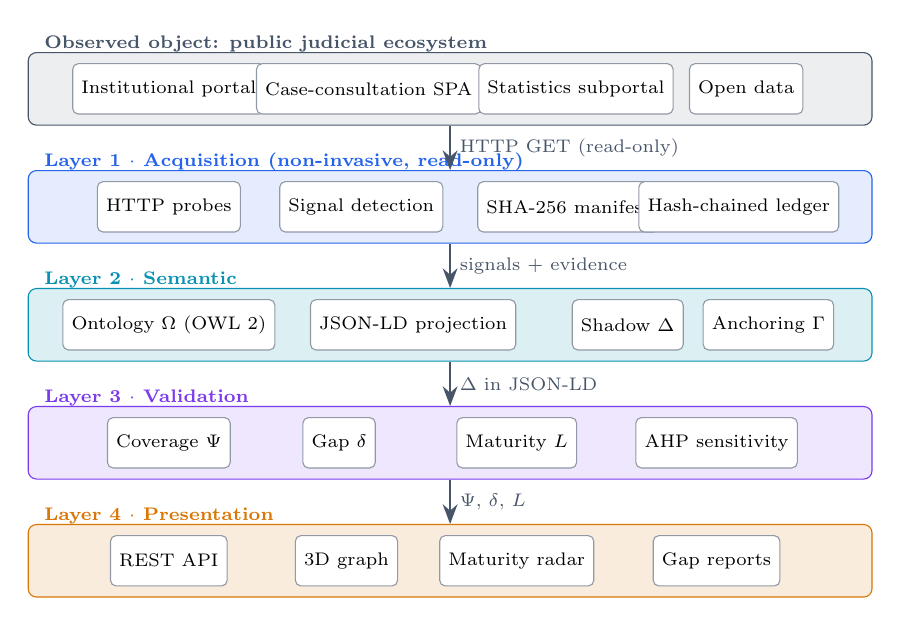
\begin{tikzpicture}[scale=0.94, transform shape,
  capa/.style={draw, rounded corners=3pt, minimum width=11.4cm, minimum height=0.98cm, align=center, font=\small},
  comp/.style={draw=lsSlate!60, rounded corners=2pt, minimum height=0.68cm, align=center, font=\scriptsize, fill=white},
  flow/.style={-{Stealth[length=2.5mm]}, thick, lsSlate}]
\node[capa, fill=lsSlate!10, draw=lsSlate] (l1) {};
\node[comp] at ($(l1.center)+(-3.8,0)$) {Institutional portal};
\node[comp] at ($(l1.center)+(-1.1,0)$) {Case-consultation SPA};
\node[comp] at ($(l1.center)+(1.7,0)$)  {Statistics subportal};
\node[comp] at ($(l1.center)+(4.0,0)$)  {Open data};
\node[font=\scriptsize\bfseries, text=lsSlate, anchor=west] at ($(l1.west)+(0.1,0.60)$) {Observed object: public judicial ecosystem};

\node[capa, below=0.60cm of l1, fill=lsBlue!12, draw=lsBlue] (l2) {};
\node[comp] at ($(l2.center)+(-3.8,0)$) {HTTP probes};
\node[comp] at ($(l2.center)+(-1.2,0)$) {Signal detection};
\node[comp] at ($(l2.center)+(1.6,0)$)  {SHA-256 manifest};
\node[comp] at ($(l2.center)+(3.9,0)$)  {Hash-chained ledger};
\node[font=\scriptsize\bfseries, text=lsBlue, anchor=west] at ($(l2.west)+(0.1,0.60)$) {Layer 1 $\cdot$ Acquisition (non-invasive, read-only)};

\node[capa, below=0.60cm of l2, fill=lsCyan!14, draw=lsCyan] (l3) {};
\node[comp] at ($(l3.center)+(-3.8,0)$) {Ontology $\Omega$ (OWL 2)};
\node[comp] at ($(l3.center)+(-0.5,0)$) {JSON-LD projection};
\node[comp] at ($(l3.center)+(2.4,0)$)  {Shadow $\Delta$};
\node[comp] at ($(l3.center)+(4.3,0)$)  {Anchoring $\Gamma$};
\node[font=\scriptsize\bfseries, text=lsCyan, anchor=west] at ($(l3.west)+(0.1,0.60)$) {Layer 2 $\cdot$ Semantic};

\node[capa, below=0.60cm of l3, fill=lsViolet!12, draw=lsViolet] (l4) {};
\node[comp] at ($(l4.center)+(-3.8,0)$) {Coverage $\Psi$};
\node[comp] at ($(l4.center)+(-1.5,0)$) {Gap $\delta$};
\node[comp] at ($(l4.center)+(0.9,0)$)  {Maturity $L$};
\node[comp] at ($(l4.center)+(3.6,0)$)  {AHP sensitivity};
\node[font=\scriptsize\bfseries, text=lsViolet, anchor=west] at ($(l4.west)+(0.1,0.60)$) {Layer 3 $\cdot$ Validation};

\node[capa, below=0.60cm of l4, fill=lsAmber!14, draw=lsAmber] (l5) {};
\node[comp] at ($(l5.center)+(-3.8,0)$) {REST API};
\node[comp] at ($(l5.center)+(-1.4,0)$) {3D graph};
\node[comp] at ($(l5.center)+(0.9,0)$)  {Maturity radar};
\node[comp] at ($(l5.center)+(3.6,0)$)  {Gap reports};
\node[font=\scriptsize\bfseries, text=lsAmber, anchor=west] at ($(l5.west)+(0.1,0.60)$) {Layer 4 $\cdot$ Presentation};

\draw[flow] (l1) -- node[right, font=\scriptsize]{HTTP GET (read-only)} (l2);
\draw[flow] (l2) -- node[right, font=\scriptsize]{signals + evidence} (l3);
\draw[flow] (l3) -- node[right, font=\scriptsize]{$\Delta$ in JSON-LD} (l4);
\draw[flow] (l4) -- node[right, font=\scriptsize]{$\Psi$, $\delta$, $L$} (l5);
\end{tikzpicture}
\caption{LegalShadow reference architecture. The flow is unidirectional from the observed ecosystem to presentation, consistent with the digital shadow definition: there is no automatic actuation on institutional infrastructure.\label{fig:arch}}
\end{figure}

\subsection{Non-Invasive Acquisition Protocol}
The acquisition module executes read-only HTTP probes against a configurable set of public targets declared in a versioned seed file. Following the ethical and legal recommendations of the literature \cite{Krotov2020}, the agent (i) identifies itself with an explicit \emph{User-Agent} stating its purpose, (ii) accesses only public resources without authentication, (iii) submits no forms and performs no write actions, (iv) caps each response at 400~KB with a 10--12~s timeout, and (v) records every capture with a UTC timestamp and a SHA-256 checksum to guarantee evidentiary traceability. Every run, verification and methodological decision is written to an append-only, hash-chained ledger, so that a third party can re-execute the capture at a new cut-off date, verify that cited snapshots were not altered, and audit the full chronology of decisions.

Deterministic \emph{signals} are then computed from the markup: generating technology, presence of legacy links (JSF/PHP extensions), SPA confirmation, references to open data and integrity policies, and---crucially---presence or absence of embedded structured data (JSON-LD/\texttt{schema.org} \cite{Guha2016}) and of a documented public API.

\subsection{Semantic Projection to JSON-LD}
Signals are projected into a JSON-LD instance whose \texttt{@context} header (Table~\ref{tab:context}) reuses standard vocabularies (Dublin Core, SKOS, Schema.org) and defines the \texttt{maltg:} namespace for governance terms. The choice of JSON-LD follows three criteria derived from the literature: native compatibility with the web development ecosystem \cite{Guha2016}, gateway status into the linked data model \cite{Bizer2009,Hitzler2021}, and alignment with FAIR interoperability and reusability principles \cite{Wilkinson2016}. Each detected component is serialised with its layer, its evidence (URL, HTTP status, size, latency), its findings and gaps, and its anchoring $\Gamma$ through \texttt{maltg:mapsTo}, turning the shadow into a queryable knowledge subgraph \cite{Hogan2021}.

\begin{table}[H]
\small
\caption{JSON-LD context of the digital shadow (extract). Artefact terms resolve to IRIs of standard vocabularies or of the project namespace.\label{tab:context}}
\begin{tabularx}{\textwidth}{llX}
\toprule
\textbf{Term} & \textbf{IRI / prefix} & \textbf{Semantic role}\\
\midrule
\texttt{maltg:} & \texttt{http://maltg.arch/onto\#} & LegalTech governance ontology (classes and properties).\\
\texttt{sdt:} & \texttt{http://maltg.arch/sdt\#} & Structural vocabulary of the shadow (components, flows).\\
\texttt{schema:} & \texttt{http://schema.org/} & Interoperability with web structured data \cite{Guha2016}.\\
\texttt{dcterms:} & \texttt{http://purl.org/dc/terms/} & Title and description metadata.\\
\texttt{skos:} & \texttt{http://www.w3.org/2004/02/skos/core\#} & Preferred concept labelling.\\
\texttt{score} & \texttt{maltg:maturityScore} & Maturity score $\sigma$ of a component or dimension.\\
\texttt{evidence} & \texttt{sdt:evidence} & Observation evidence (URL, status, latency, hash).\\
\texttt{maltg\_ref} & \texttt{maltg:mapsTo} (\texttt{@type=@id}) & Semantic anchoring $\Gamma$ towards concepts of $\Omega$.\\
\texttt{services} & \texttt{sdt:hasComponent} & Vertices $V$ of the graph $\Delta$.\\
\texttt{connections} & \texttt{sdt:hasFlow} & Edges $E$ of the graph $\Delta$.\\
\bottomrule
\end{tabularx}
\end{table}

\subsection{Evaluation Cycle}
After each ingestion the validation layer computes Equations~\eqref{eq:coverage-set}--\eqref{eq:global} and persists the dated shadow, producing a time series of artefacts comparable across institutions and across dates. The cycle design is inspired by the MAPE-K loop of autonomic computing \cite{Kephart2003}---monitor, analyse, plan and execute over a shared knowledge base---with the deliberate caveat that the execution phase is restricted to recommendations: closing the loop on the observed system is the institution's prerogative. This restriction is the architectural translation of the artefact's \emph{shadow} (rather than twin) character \cite{Kritzinger2018,Sepasgozar2021}.

%% ============================================================
\section{Case Study and Results}
\label{sec:results}

\subsection{Experimental Design}
Validation comprises three complementary elements. \textbf{(A)} An institutional case study on the public digital ecosystem of the Ecuadorian Judiciary Council (\texttt{funcionjudicial\-.gob\-.ec}), producing dated shadows with four diagnostic maturity dimensions. \textbf{(B)} A ten-dimension semantic validation of the same real shadow against the full ontology $\Omega$ (131 classes, 144 relations, 14 of them cross-cutting), contrasted with a synthetic control shadow of 39 components purposely built to saturate the engine. \textbf{(C)} A cross-institutional portability probe. All reported figures were regenerated from the persisted artefacts; the ontology digest is \texttt{5130ea40119d} and the shadow digest \texttt{8156a9e3de28}.

\subsection{Experimental Apparatus}
\label{sec:apparatus}
The experiments were conducted through two instrumented consoles of the containerised platform, which correspond to the acquisition and validation layers of Figure~\ref{fig:arch}.

The \textbf{GET-SDS console} implements the acquisition experiment. It takes a configurable target URL, executes the read-only protocol of Section~\ref{sec:arch}, and renders the ontology $\Omega$ as a three-dimensional star field in which each class is a star and each architectural layer a constellation. The field starts uniformly dim; as the scan proceeds, every ontological term is matched against the evidence gathered from the target and the corresponding star is lit only if evidence supports it. The lit subset is a direct visual instantiation of the coverage set $R$ of Equation~\eqref{eq:coverage-set}, and a live inspection panel reports the running count of evidenced nodes. This makes the otherwise abstract anchoring function $\Gamma$ observable during the experiment and, because the target URL is a parameter rather than a constant, it is also the mechanism through which the portability probe of Element C was run.

The \textbf{SDS console} implements the validation experiment. It loads any shadow present in the artefact repository through a selector, recomputes Equations~\eqref{eq:psi}--\eqref{eq:global} against the current ontology, and reports the maturity radar, the per-dimension table of $\mathrm{onto}(d)$, $\mathrm{sds}(d)$, $\delta(d)$ and coverage percentage, the ranked top-gap list, and the findings and gaps recorded for each governance dimension together with the component and source inventory. Because the engine is shadow-agnostic, the same code path evaluates the real institutional shadow and the synthetic control, which is what makes the contrast of Section~\ref{sec:elementB} methodologically sound: the two figures differ only in their input artefact.


Figure~\ref{fig:getsds} renders that process. The target URL is a parameter; the protocol yields signals and hashed snapshots; the signals are projected into the JSON-LD shadow; and the anchoring $\Gamma$ decides, class by class, which of the 131 ontological stars are lit. The console displays the ontology as a rotating sphere in which the 144 relations form the edges and each cluster of classes---TOGAF, COBIT, ITIL, NIST CSF, AI, DLT, open data, security, LegalTech---forms a named constellation, so the coverage set $R$ of Equation~\eqref{eq:coverage-set} is read off directly as the lit fraction of the sphere.

\begin{figure}[H]
\centering
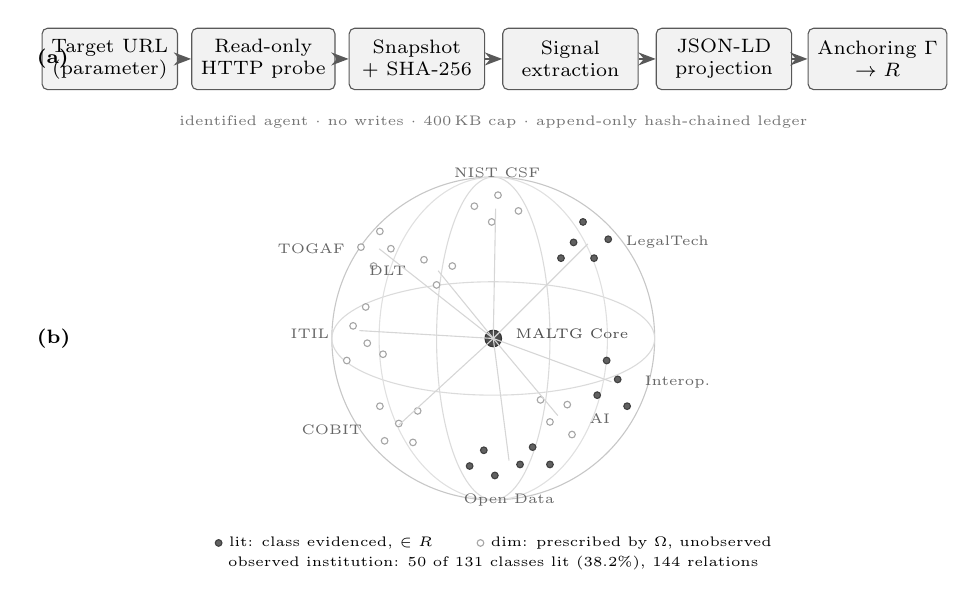
\begin{tikzpicture}[
  stg/.style={draw=black!65, rounded corners=2pt, minimum width=1.72cm, minimum height=0.78cm, align=center, font=\scriptsize, fill=black!5},
  arr/.style={-{Stealth[length=2.2mm]}, thick, black!65},
  lit/.style={circle, fill=black!62, draw=black!75, inner sep=0pt, minimum size=2.4pt},
  dim/.style={circle, fill=white, draw=black!35, inner sep=0pt, minimum size=2.4pt},
  cst/.style={font=\tiny, text=black!60}]

%% ── (a) pipeline ─────────────────────────────────────────
\node[stg] (s0) at (0,0)    {Target URL\\\scriptsize(parameter)};
\node[stg] (s1) at (1.95,0) {Read-only\\HTTP probe};
\node[stg] (s2) at (3.90,0) {Snapshot\\+ SHA-256};
\node[stg] (s3) at (5.85,0) {Signal\\extraction};
\node[stg] (s4) at (7.80,0) {JSON-LD\\projection};
\node[stg] (s5) at (9.75,0) {Anchoring $\Gamma$\\$\rightarrow R$};
\foreach \a/\b in {s0/s1,s1/s2,s2/s3,s3/s4,s4/s5}{\draw[arr] (\a) -- (\b);}
\node[font=\tiny, text=black!55, anchor=north] at (4.87,-0.60)
  {identified agent $\cdot$ no writes $\cdot$ 400\,KB cap $\cdot$ append-only hash-chained ledger};
\node[font=\scriptsize\bfseries, anchor=west] at (-1.05,0) {(\textbf{a})};

%% ── (b) constellation ────────────────────────────────────
\begin{scope}[shift={(4.87,-3.55)}]
\draw[black!22] (0,0) circle (2.05);
\draw[black!14] (0,0) ellipse (2.05 and 0.72);
\draw[black!14] (0,0) ellipse (0.72 and 2.05);
\draw[black!12] (0,0) ellipse (1.45 and 2.05);
\node[circle, fill=black!70, draw=black!80, inner sep=0pt, minimum size=6pt] (core) at (0,0) {};
\node[font=\tiny, text=black!70, anchor=west] at (0.16,0.055) {MALTG Core};

%% lit constellations (evidenced clusters)
\foreach \x/\y in {-0.30/-1.62, 0.02/-1.74, 0.34/-1.60, -0.12/-1.42, 0.50/-1.38, 0.72/-1.60}
  {\node[lit] at (\x,\y) {};}
\node[cst, anchor=north] at (0.2,-1.85) {Open Data};
\foreach \x/\y in {1.32/-0.72, 1.58/-0.52, 1.44/-0.28, 1.70/-0.86}{\node[lit] at (\x,\y) {};}
\node[cst, anchor=west] at (1.80,-0.55) {Interop.};
\foreach \x/\y in {1.02/1.22, 1.28/1.02, 1.46/1.26, 1.14/1.48, 0.86/1.02}{\node[lit] at (\x,\y) {};}
\node[cst, anchor=west] at (1.56,1.22) {LegalTech};

%% dim constellations (prescribed, unobserved)
\foreach \x/\y in {-1.52/0.92, -1.30/1.14, -1.68/1.16, -1.44/1.36}{\node[dim] at (\x,\y) {};}
\node[cst, anchor=east] at (-1.76,1.14) {TOGAF};
\foreach \x/\y in {-1.78/0.16, -1.60/-0.06, -1.86/-0.28, -1.62/0.40, -1.40/-0.20}{\node[dim] at (\x,\y) {};}
\node[cst, anchor=east] at (-1.96,0.06) {ITIL};
\foreach \x/\y in {-1.20/-1.08, -1.44/-0.86, -1.02/-1.32, -1.38/-1.30, -0.96/-0.92}{\node[dim] at (\x,\y) {};}
\node[cst, anchor=east] at (-1.54,-1.16) {COBIT};
\foreach \x/\y in {-0.24/1.68, 0.06/1.82, 0.32/1.62, -0.02/1.48}{\node[dim] at (\x,\y) {};}
\node[cst, anchor=south] at (0.05,1.92) {NIST CSF};
\foreach \x/\y in {0.72/-1.06, 0.94/-0.84, 0.60/-0.78, 1.00/-1.22}{\node[dim] at (\x,\y) {};}
\node[cst, anchor=west] at (1.10,-1.02) {AI};
\foreach \x/\y in {-0.72/0.68, -0.52/0.92, -0.88/1.00}{\node[dim] at (\x,\y) {};}
\node[cst, anchor=east] at (-0.98,0.86) {DLT};

\foreach \p in {(0.2,-1.55),(1.5,-0.55),(1.2,1.2),(-1.45,1.14),(-1.7,0.10),(-1.2,-1.10),(0.03,1.65),(0.82,-0.98),(-0.7,0.86)}
  {\draw[black!16] (0,0) -- \p;}
\end{scope}
\node[font=\scriptsize\bfseries, anchor=west] at (-1.05,-3.55) {(\textbf{b})};
\node[font=\tiny, anchor=north, align=center] at (4.87,-5.95)
  {\tikz\node[lit]{};~lit: class evidenced, $\in R$ \qquad \tikz\node[dim]{};~dim: prescribed by $\Omega$, unobserved\\[1pt]
   observed institution: 50 of 131 classes lit (38.2\%), 144 relations};
\end{tikzpicture}
\caption{The GET-SDS acquisition process. (\textbf{a}) The non-invasive pipeline, from a parameterised target URL to the coverage set $R$. (\textbf{b}) The ontology rendered as a celestial sphere: each class is a star, each governance cluster a named constellation. The sphere starts uniformly dim and a scan lights only the classes for which evidence was found, making the anchoring function $\Gamma$ and the coverage set $R$ directly observable. Open data, interoperability and the LegalTech domain light up; TOGAF, COBIT, ITIL, NIST CSF, AI and DLT remain dim.\label{fig:getsds}}
\end{figure}

For the shadow of 4 August 2026, anchoring is \emph{total and referentially closed}: all 34 components carry at least one anchor (mean 2.00, maximum 4 per component) and all 50 distinct references resolve to existing ontology classes, with zero dangling identifiers. The constellation therefore lights 50 of the 131 ontological stars, i.e.\ 38.2\% of the conceptual space.

\subsection{Evidence Corpus and Reproducibility}
Table~\ref{tab:corpus} summarises the acquisition corpus. Over 17 dated runs between 2 July and 4 August 2026 the module issued 187 read-only requests, of which 170 succeeded (90.9\%). Re-hashing every stored snapshot and comparing against its manifest yields \textbf{170 matches and 0 mismatches}, i.e.\ full integrity of the evidence base. The ledger holds 37 chained entries from \texttt{GENESIS} to head \texttt{6c7d2847932a606f}. Observed latencies (median 788.5~ms, p95 954.4~ms) confirm that the probe imposes a negligible load on the observed infrastructure, which is a design requirement of the ethical protocol \cite{Krotov2020}.

\begin{table}[H]
\small
\caption{Acquisition corpus and reproducibility indicators (2 July--4 August 2026).\label{tab:corpus}}
\begin{tabularx}{\textwidth}{Xcc}
\toprule
\textbf{Indicator} & \textbf{Value} & \textbf{Role}\\
\midrule
Dated acquisition runs & 17 & Longitudinal comparability.\\
Read-only requests issued & 187 & Observation effort.\\
Successful captures & 170 (90.9\%) & Availability of public sources.\\
Snapshots re-verified by SHA-256 & 170 / 170 & Evidence integrity.\\
Hash mismatches detected & 0 & No tampering or drift in stored evidence.\\
Ledger entries (append-only, chained) & 37 & Auditable chronology of decisions.\\
Response latency: median / p95 & 788.5 / 954.4 ms & Non-invasiveness of the probe.\\
Latency range (min--max) & 67--2810 ms & Heterogeneity of the ecosystem.\\
\bottomrule
\end{tabularx}
\end{table}

\subsection{Element A: Institutional Shadow and Declarative Maturity}
The shadow generated from the 4 August 2026 run contains \textbf{34 components, 32 flows and 7 architectural layers}, anchored to 11 seed sources. Table~\ref{tab:signals} lists the observation signals. Three structural findings stand out: a modern portal built on a generic content management system that still surfaces 16 legacy links (6 JSF and 10 PHP); a confirmed case-consultation SPA with no documented public API; and the total absence of embedded JSON-LD structured data, despite declarative references to open data policies---exactly the gap between nominal publication and effective reuse described in the open government literature \cite{Janssen2012,Attard2015}.

\begin{table}[H]
\small
\caption{Observation signals of the judicial ecosystem (run of 4 August 2026; identified agent, read-only).\label{tab:signals}}
\begin{tabularx}{\textwidth}{Xcc}
\toprule
\textbf{Signal} & \textbf{Value} & \textbf{Governance implication}\\
\midrule
Portal online (HTTP 200) & Yes & Citizen channel available.\\
Generic CMS confirmed & Yes & Dependence on a non-specialised platform.\\
Legacy JSF links & 6 & Technical debt visible on the public surface.\\
Legacy PHP links & 10 & Technological fragmentation.\\
Case-consultation SPA confirmed & Yes & Partial front-end modernisation.\\
Open data reference & Yes & Declarative commitment present.\\
Anti-bribery standard reference (ISO 37001) & Yes & Declarative compliance signal.\\
JSON-LD / \texttt{schema.org} detected & \textbf{No} & No semantic web exposure.\\
Documented public API & \textbf{No} & Programmatic reuse blocked.\\
\bottomrule
\end{tabularx}
\end{table}

The four-dimension institutional assessment (Table~\ref{tab:cjdims}, Figure~\ref{fig:radar}) yields a global maturity index of \textbf{46/100}, which $L$ places at Level 3 (``Defined''). The weakest dimension is the data and semantic interoperability layer (28/100), consistent with the negative JSON-LD and API signals; the strongest is declarative regulatory compliance (58/100), driven by the detected normative references. The index proved stable across all five regenerated shadows in the series, the only signal drift being the legacy PHP link count (13 $\rightarrow$ 10 between 5 and 30 July 2026), which the protocol attributes to content editing on the observed portal rather than to observer variance.

\begin{table}[H]
\small
\caption{Maturity dimensions of the institutional digital shadow.\label{tab:cjdims}}
\begin{tabularx}{\textwidth}{Xccc}
\toprule
\textbf{Dimension} & \textbf{Score} & \textbf{Findings} & \textbf{Gaps}\\
\midrule
Data and semantic interoperability layer & 28 & 2 & 3\\
Integration architecture (API and front-end) & 42 & 2 & 3\\
Declared transformation and innovation & 55 & 2 & 2\\
Regulatory compliance and automation & 58 & 3 & 2\\
\midrule
\textbf{Global index (mean)} & \textbf{46} & \multicolumn{2}{c}{Level 3 $\cdot$ Defined}\\
\bottomrule
\end{tabularx}
\end{table}

\begin{figure}[H]
\centering
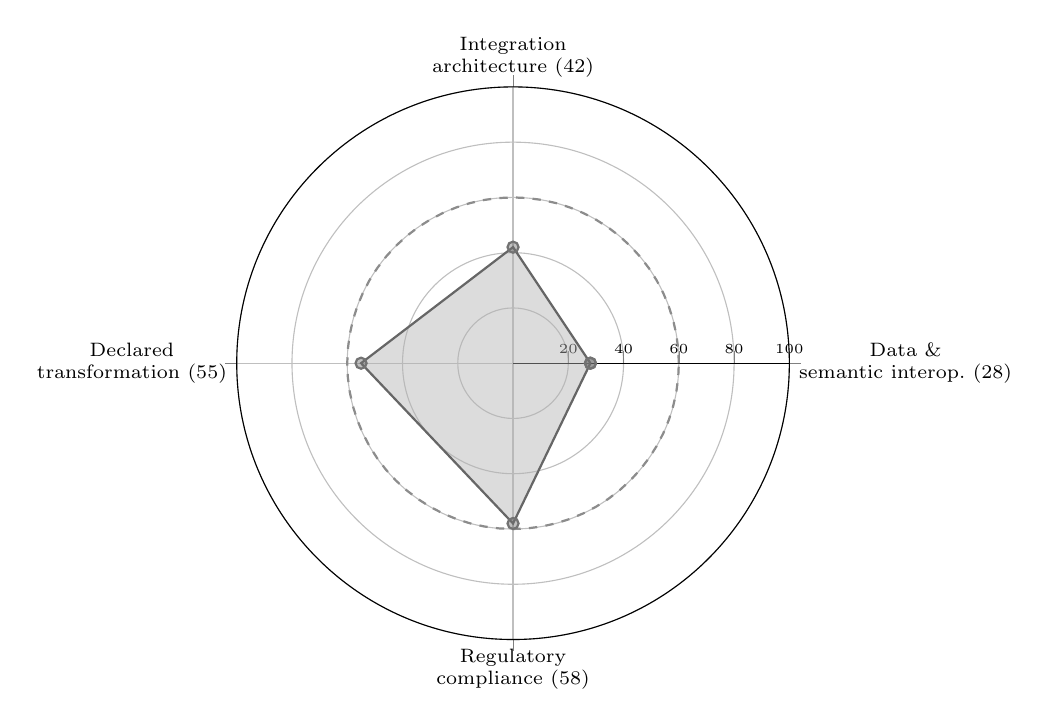
\begin{tikzpicture}
\begin{polaraxis}[
  width=8.6cm,
  xtick={0,90,180,270},
  xticklabels={
    {Data \&\\semantic interop.\ (28)},
    {Integration\\architecture (42)},
    {Declared\\transformation (55)},
    {Regulatory\\compliance (58)}},
  xticklabel style={font=\scriptsize, align=center},
  ytick={20,40,60,80,100},
  yticklabel style={font=\tiny},
  ymin=0, ymax=100,
  grid=both,
  major grid style={black!25},
]
\addplot+[thick, mark=*, mark options={fill=black!55, draw=black!55}, fill=black!30, fill opacity=0.45, draw=black!60]
  coordinates {(0,28) (90,42) (180,55) (270,58) (360,28)};
\addplot+[thick, dashed, no marks, domain=0:360, samples=73, draw=black!45]{60};
\end{polaraxis}
\end{tikzpicture}
\caption{Maturity radar of the four institutional dimensions. The dashed line marks the Level 4 threshold (``Managed'', 61+). The observed polygon (mean 46/100) exposes the lag of semantic interoperability.\label{fig:radar}}
\end{figure}

\subsection{Element B: Ten-Dimension Semantic Validation}
\label{sec:elementB}
Applying the engine of Section~\ref{sec:formal} to the \emph{same real shadow} against the full ontology produces the results in Table~\ref{tab:validation} and Figure~\ref{fig:gaps}. Global coverage is
\[
\Psi_{\mathrm{global}} \;=\; \frac{\mathrm{SDS}_{\mathrm{global}}}{\mathrm{Onto}_{\mathrm{global}}} \;=\; \frac{25.8}{73.9} \;=\; 0.349,
\]
that is, the observed shadow materialises only \textbf{34.9\%} of the maturity prescribed by the ontology, leaving an aggregate gap of 48.1 points (65.1\%). By contrast, the synthetic control shadow---built to exercise every dimension---reaches $\Psi_{\mathrm{global}}=66.9/73.9=90.5\%$ with a residual gap of 7.0 points. The control therefore confirms that the low real coverage is a property of the observed ecosystem and not an artefact of the engine.

A result that only the shared apparatus of Section~\ref{sec:apparatus} makes visible is that the two shadows light an almost identical number of stars---50 of 131 for the real shadow against 51 of 131 for the control---yet their global coverage differs by a factor of 2.6 ($34.9\%$ versus $90.5\%$). Coverage breadth is therefore not what $\Psi$ measures: \emph{which} concepts are anchored matters far more than how many. The control distributes its 51 anchors across all ten dimensions, whereas the real ecosystem concentrates its 50 anchors in open data, interoperability and the LegalTech domain, leaving whole dimensions untouched. A naive count of evidenced ontology nodes would have rated the two artefacts as equivalent; the hierarchical decomposition of Equation~\eqref{eq:psi} separates them.

Three dimensions have \emph{zero or near-zero} coverage because neither their root nor their subconcepts appear in $R$: service management (ITIL, $\delta=79.5$), control (COBIT, $\delta=62.7$) and distributed ledger (BC, $\delta=52.4$). The single largest gap is AI integration ($\delta=82.4$), where the high ontological score (96.9) is almost entirely unrealised: only one of four subconcepts is anchored. Conversely, open data attains full coverage ($\Psi=1.00$) and interoperability reaches 0.85, reflecting the institution's genuine participation in the national open data catalogue. This is the paper's central empirical contrast: an institution that self-reports a ``Defined'' maturity of 46/100 on declarative dimensions materialises barely a third of the governance semantics that the same framework prescribes.

\begin{table}[H]
\small
\caption{Hierarchical coverage validation of the real institutional shadow (Element B), $(w_r,w_s)=(0.40,\,0.60)$. $\mathrm{onto}(d)$: ontological maturity; $\Psi(d)$: coverage; $\mathrm{sds}(d)$: effective shadow maturity; $\delta(d)$: gap. The rightmost column reports the synthetic control for the same dimension.\label{tab:validation}}
\begin{adjustwidth}{-\extralength}{0cm}
\begin{tabularx}{\fulllength}{Xccccccc}
\toprule
\textbf{Dimension} & $\mathbf{onto(d)}$ & \textbf{Root} & $\mathbf{\Psi(d)}$ & $\mathbf{sds(d)}$ & $\boldsymbol{\delta}\mathbf{(d)}$ & \textbf{Missing subs} & $\mathbf{\Psi}$ \textbf{control}\\
\midrule
AI integration              & 96.9 & No  & 0.15 & 14.5 & \textbf{82.4} & 3 of 4 & 0.85\\
Service management (ITIL)   & 79.5 & No  & 0.00 & 0.0  & \textbf{79.5} & 5 of 5 & 1.00\\
Resilience (NIST CSF)       & 72.0 & No  & 0.12 & 8.6  & 63.4 & 4 of 5 & 1.00\\
Control (COBIT)             & 62.7 & No  & 0.00 & 0.0  & 62.7 & 5 of 5 & 1.00\\
Security posture            & 80.4 & No  & 0.30 & 24.1 & 56.3 & 2 of 4 & 1.00\\
Distributed ledger          & 52.4 & No  & 0.00 & 0.0  & 52.4 & 4 of 4 & 0.85\\
Governance (TOGAF)          & 60.3 & No  & 0.20 & 12.1 & 48.2 & 4 of 6 & 0.70\\
LegalTech domain            & 75.5 & Yes & 0.67 & 50.8 & 24.7 & 6 of 11 & 0.60\\
Interoperability            & 81.2 & Yes & 0.85 & 69.0 & 12.2 & 2 of 8 & 1.00\\
Open data                   & 78.5 & Yes & 1.00 & 78.5 & 0.0  & 0 of 4 & 1.00\\
\midrule
\textbf{Global (simple mean)} & \textbf{73.9} & 3/10 & \textbf{0.349} & \textbf{25.8} & \textbf{48.1} & --- & \textbf{0.905}\\
\bottomrule
\end{tabularx}
\end{adjustwidth}
\end{table}

\begin{figure}[H]
\begin{adjustwidth}{-\extralength}{0cm}
\centering
\begin{tikzpicture}
\begin{axis}[
  ybar,
  width=\fulllength, height=6.4cm,
  bar width=6pt,
  ymin=0, ymax=112,
  ylabel={Score (0--100)},
  ylabel style={font=\small},
  symbolic x coords={AI,ITIL,NIST,COBIT,Security,DLT,TOGAF,LegalTech,Interop.,Open data},
  xtick=data,
  x tick label style={rotate=32, anchor=east, font=\scriptsize},
  ytick={0,20,40,60,80,100},
  yticklabel style={font=\scriptsize},
  legend style={font=\scriptsize, at={(0.5,1.02)}, anchor=south, legend columns=3, draw=none},
  ymajorgrids, major grid style={black!20},
]
\addplot+[draw=lsBlue!80!black, fill=lsBlue!35] coordinates
  {(AI,96.9) (ITIL,79.5) (NIST,72.0) (COBIT,62.7) (Security,80.4) (DLT,52.4) (TOGAF,60.3) (LegalTech,75.5) (Interop.,81.2) (Open data,78.5)};
\addplot+[draw=black, fill=black!62] coordinates
  {(AI,14.5) (ITIL,0) (NIST,8.6) (COBIT,0) (Security,24.1) (DLT,0) (TOGAF,12.1) (LegalTech,50.8) (Interop.,69.0) (Open data,78.5)};
\addplot[sharp plot, very thick, dashed, black, mark=*, mark size=1.4pt, mark options={fill=black,draw=black}] coordinates
  {(AI,82.4) (ITIL,79.5) (NIST,63.4) (COBIT,62.7) (Security,56.3) (DLT,52.4) (TOGAF,48.2) (LegalTech,24.7) (Interop.,12.2) (Open data,0)};
\legend{$\mathrm{onto}(d)$ ontology, $\mathrm{sds}(d)$ observed shadow, $\delta(d)$ gap}
\end{axis}
\end{tikzpicture}
\end{adjustwidth}
\caption{Ontological maturity versus effective maturity of the real institutional shadow, by dimension, ordered by decreasing gap. The dashed line traces $\delta(d)$ and constitutes the remediation agenda: AI integration, service management and resilience concentrate the deficit, whereas open data is fully covered.\label{fig:gaps}}
\end{figure}

\subsection{Sensitivity Analysis}
Since $\Psi$ depends on the weights $(w_r,w_s)$, robustness of the gap ordering was assessed by sweeping $w_r \in [0.10,0.90]$ (Table~\ref{tab:sensitivity}). By Equation~\eqref{eq:psi}, $\Psi(d)$ is linear in $w_r$ for each dimension, so the relative ordering of $\delta$ can only change where lines cross. The global shadow score varies monotonically but narrowly, from 26.9 to 23.9 (a span of 3.0 points on a 100-point scale), and the aggregate gap stays within 63.6--67.7\%. AI integration and service management occupy the top two positions of the remediation agenda across the entire interval, exchanging rank only at $w_r \leq 0.20$. The conclusion is that the prioritisation delivered to decision makers is insensitive to reasonable variation of expert judgement, which strengthens the practical utility of AHP calibration \cite{Saaty1990}.

\begin{table}[H]
\small
\caption{Sensitivity of the global result and of the remediation agenda to the root weight $w_r$.\label{tab:sensitivity}}
\begin{tabularx}{\textwidth}{cccX}
\toprule
$\mathbf{w_r}$ & $\mathbf{SDS_{global}}$ & \textbf{Gap (\%)} & \textbf{Top-3 remediation agenda}\\
\midrule
0.10 & 26.9 & 63.6 & ITIL, AI, COBIT\\
0.20 & 26.5 & 64.1 & ITIL, AI, COBIT\\
0.30 & 26.1 & 64.7 & AI, ITIL, COBIT\\
0.40 (default) & 25.8 & 65.1 & AI, ITIL, NIST\\
0.50 & 25.4 & 65.6 & AI, ITIL, NIST\\
0.60 & 25.0 & 66.2 & AI, ITIL, NIST\\
0.70 & 24.6 & 66.7 & AI, ITIL, Security\\
0.80 & 24.3 & 67.1 & AI, ITIL, Security\\
0.90 & 23.9 & 67.7 & AI, ITIL, Security\\
\bottomrule
\end{tabularx}
\end{table}

\subsection{Element C: Cross-Institutional Portability}
To test that neither the protocol nor the signal vocabulary is bound to a single institution, the acquisition procedure was executed unchanged against a second Ecuadorian judicial body, the Constitutional Court (\texttt{corteconstitucional\-.gob\-.ec}), on 7 August 2026. The probe returned a clearly distinct signal profile: a different generating technology (\texttt{Divi Child v.1.0.0} versus the Elementor-based stack of the first institution), 40 PHP legacy references but no JSF references, 73 outbound links, a 741~KB document, and---unlike the first institution---\textbf{one embedded JSON-LD block}. That a single, unmodified probe discriminates between two institutions on the very signal that drives the weakest dimension (semantic exposure) is evidence that the instrument measures an institutional property rather than a constant of the domain.

Two caveats must be stated explicitly. First, this probe rendered the DOM through a browser engine, whereas the corpus of Table~\ref{tab:corpus} used raw HTTP snapshots; raw counts are therefore comparable in kind but not numerically commensurable across the two channels. Second, a full second-institution shadow with its own $\Psi/\delta$ evaluation was not produced, so no maturity ranking between institutions is claimed here. Element C establishes portability of the acquisition layer, not a comparative maturity result.

\subsection{Partial Empirical Closure}
The architecture also admits a partial empirical closure of the LegalTech dimension. A symbolic reasoner over 47 real case files, evaluating procedural acts against statutory terms and the judicial holiday calendar, produced an empirical health index of 36.7/100 (22 of 60 evaluable acts within term). Blending it with the declarative score at equal weight lowers the LegalTech dimension from 50.8 to 43.8: the declarative assessment overstates that dimension by 16\% relative to observed procedural behaviour. This is a first, deliberately conservative step towards connecting the structural shadow with the behaviour of the justice system.

%% ============================================================
\section{Discussion}
\label{sec:discussion}

\textbf{Declarative maturity is not machine-actionable governance.} The juxtaposition of Elements A and B is the paper's main result. On its own declarative dimensions the institution scores 46/100 (Level 3, ``Defined''), a figure that a conventional maturity assessment would report as reasonable progress. Evaluated against the semantics of the same governance frameworks it invokes, the observable ecosystem materialises only 34.9\% of the prescribed maturity, and three of ten dimensions have literally zero anchored concepts. The instrument thus separates two things that maturity questionnaires conflate: what an institution \emph{declares} and what its digital surface \emph{exposes in machine-processable form}.

\textbf{A reflexive finding.} The most deficient signal is precisely the absence of JSON-LD and of a public API. The observed institution therefore lacks the very instrument---structured data---that the digital shadow uses to represent it. Institutional adoption of semantic markup would, besides improving findability \cite{Guha2016}, directly lift the weakest dimension of the radar and enable third parties (academia, civil society) to build value-added services on judicial data \cite{Attard2015}, in line with FAIR principles \cite{Wilkinson2016}.

\textbf{Contribution to the open validation problem.} Karabulut et al. identify the absence of methods to verify that a digital twin actually materialises its semantic model \cite{Karabulut2024}. The function $\Psi$ offers an operational answer: computable in linear time, bounded, monotone and interpretable dimension by dimension, it enables continuous audits of ontology--artefact alignment, and its root/subconcept decomposition localises the origin of the deficit. The contrast within Table~\ref{tab:validation} between ITIL ($\mathbb{1}[r_d \in R]=0$ and $S_d \cap R = \emptyset$, a dimension entirely absent) and interoperability (root covered, two subconcepts missing, a dimension merely incomplete) illustrates a diagnostic distinction that a scalar score cannot express.

\textbf{Generalisation.} Although the case study is Ecuadorian, no element of the architecture is country-specific: the ontology encodes international frameworks, the protocol operates over standard HTTP, and the JSON-LD context reuses global vocabularies. Element C shows the probe runs unchanged on a second institution and discriminates between them. Dated shadows per institution therefore enable longitudinal comparison (one judiciary over time) and cross-sectional comparison (regional maturity ranking), extending to justice the logic of comparable urban twins \cite{Shahat2021}.

\textbf{Limitations and threats to validity.} The most consequential limitation is that the shadow observes only the \emph{public surface} of the ecosystem: scores are \emph{observable} maturity, a lower bound on real maturity, and dimensions such as ITIL or COBIT may well operate internally without public trace, so their zero coverage measures published evidence rather than practice. Further, the scores $\sigma$ and weights $(w_r,w_s,\omega_d)$ embed expert judgement---mitigated by Lawshe's CVR \cite{Lawshe1975}, AHP calibration \cite{Saaty1990} and the sensitivity analysis of Table~\ref{tab:sensitivity}, but not eliminated---and global aggregation uses a simple mean for want of a validated Delphi panel. Finally, external validity is limited to one institution studied in depth plus a single probe of a second, and signal detection depends on the stability of portal markup; the cryptographic record attenuates, without eliminating, observer drift, as the documented 13~$\rightarrow$~10 PHP link variation shows.

%% ============================================================
\section{Conclusions}
\label{sec:conclusions}

This paper presented LegalShadow, an architecture that instantiates the digital shadow paradigm over the technological ecosystem of a judicial institution, with three distinctive properties: automatic generation from public web evidence with cryptographically verifiable provenance, semantic grounding in a multi-standard governance ontology serialised in JSON-LD, and quantitative validation through the hierarchical coverage function $\Psi$ and gap function $\delta$, whose boundedness, monotonicity and saturation were established.

The empirical study over 17 dated runs, 187 read-only requests and 170 integrity-verified snapshots (0 mismatches) produced an actionable diagnosis for the Ecuadorian Judiciary Council: a declarative maturity index of 46/100 (Level 3) coexisting with a semantic coverage of only 34.9\%, against 90.5\% for a synthetic control that saturates the engine. The remediation agenda---AI integration, service management and resilience---proved stable under variation of the root weight across $w_r \in [0.10,0.90]$. The gap between what the institution declares and what its digital surface exposes in machine-processable form is, we argue, the quantity that governance audits of digitalising judiciaries most need to measure.

Future work follows four directions: (i) multi-institutional and longitudinal studies producing full $\Psi/\delta$ evaluations per institution, so that the portability shown in Element C becomes a comparative maturity result; (ii) assisted loop closure through recommendations generated over the knowledge base while preserving human decision, following MAPE-K \cite{Kephart2003}; (iii) enrichment of the anchoring $\Gamma$ with automatic ontology alignment techniques over knowledge graphs \cite{Hogan2021}; and (iv) extension of the empirical closure sketched in Section~\ref{sec:results} into a fully-fledged behavioural dimension based on procedural performance indicators \cite{Medvedeva2020}.

\vspace{6pt}

\authorcontributions{Conceptualisation, methodology, software, validation and writing---original draft, P.M.P.-A.; supervision, formal analysis and writing---review and editing, E.J.S.-C. and V.V.V.-B. All authors have read and agreed to the published version of the manuscript.}

\funding{This research received no external funding.}

\institutionalreview{Not applicable.}

\informedconsent{Not applicable.}

\dataavailability{The LegalShadow source code, the OWL ontology, the dated JSON-LD shadows and the SHA-256 evidence manifests are available from the corresponding author on request. Observed data originate from public resources of the Ecuadorian Judiciary Council and the Constitutional Court of Ecuador.}

\conflictsofinterest{The authors declare no conflicts of interest.}

%% ============================================================
\begin{adjustwidth}{-\extralength}{0cm}
\reftitle{References}
\bibliography{references}
\end{adjustwidth}

\end{document}
